\documentclass{report}
\usepackage[T1]{fontenc} % Fontes T1
\usepackage[utf8]{inputenc} % Input UTF8
\usepackage[backend=biber, style=ieee]{biblatex} % para usar bibliografia
\usepackage{csquotes}
\usepackage[portuguese]{babel} %Usar língua portuguesa
\usepackage{blindtext} % Gerar texto automaticamente
\usepackage[printonlyused]{acronym}
\usepackage{hyperref} % para autoref
\usepackage{graphicx}

\bibliography{bibliografia}

\begin{document}
%%
% Definições
%
\def\titulo{Projeto de MPEI - Relatório}
\def\autores{93289 - Alexandre Oliveira, 95228 - Lara Matos}
\def\departamento{Departamento de Eletrónica,Telecomunicações e Informática}
\def\empresa{Universidade de Aveiro - Métodos Probabilísticos para Engenharia Informática}
\def\logotipo{ua.pdf}

%
%%%%%% CAPA %%%%%%
%
\begin{titlepage}

\begin{center}
%
\vspace*{50mm}
%
{\Huge \titulo}\\ 
%
\vspace{10mm}
%
{\Large \empresa}\\
%
\vspace{10mm}
%
{\LARGE \autores}\\ 
%
\vspace{30mm}
%
\begin{figure}[h]
\center
\includegraphics{\logotipo}
\end{figure}
%
\vspace{30mm}
\end{center}
%
\end{titlepage}

%%  Página de Título %%
\title{%
{\Huge\textbf{\titulo}}\\
{\Large \departamento\\ \empresa}
}
%
\author{%
    \autores \\
    \autorescontactos
}
%
\date{\data}
%


%%%%%%%%%%%%%%%%%%%%%%%%%%%%%%%
\clearpage
\pagenumbering{arabic}

%%%%%%%%%%%%%%%%%%%%%%%%%%%%%%%%
\chapter{Resumo}
\label{chap.resumo}

\paragraph{ }
No âmbito da unidade curricular de Métodos Probabilísticos para Engenharia Informática foi proposto aos alunos a realização de um projeto cujo objetivo principal fosse a criação de uma aplicação que utilizasse algumas matérias lecionadas durante as aulas teórico-práticas da referida disciplina. Para isso, este grupo escolheu o problema 9 (desenvolvimento de uma aplicação para uma lista de letras de músicas) com as seguintes finalidades:
\begin{itemize}
	\item Determinação das letras das músicas que contêm uma palavra específica ou um conjunto de palavras;
	\item Qual a letra mais similar a uma determinada letra;
	\item Quais os pares de letras que têm uma similaridade superior a um determinado valor.
	\end{itemize}

Para o bom funcionamento da aplicação, é recomendável o uso de algoritmos \textit{MinHash}, para a demonstração de um valor aproximado da similaridade de \textit{Jaccard}.

Neste relatório, serão abordados items relacionados com o trabalho, tais como a maneira correta de correr os programas, os módulos implementados na aplicação, os testes efetuados e os resultados desses mesmos testes.

%----------Desenvolvimento-----------%

\chapter{Como correr os programas}
\label{chap.programas}

\paragraph{}
Para a execução correta da aplicação deve-se fazer os seguintes passos:

\begin{itemize}
	\item Num terminal, abrir o diretório \texttt{Project\_MPEI\_93289\_95228} e em seguida o diretório \textit{src};
	
	\item Compilar a aplicação \textit{LetrasMusicais}: \textbf{javac LetrasMusicais.java};
	
	\item Executar a aplicação \textit{LetrasMusicais}: \textbf{java LetrasMusicais}.
\end{itemize}

Esta \textit{app} tem como função ler o ficheiro \textit{lyrics.txt} constituído por 302 letras de músicas, tendo como ficheiro principal (\textit{main}) o programa \textit{LetrasMusicais.java} com a apresentação de um menu, e vai fazer os seguintes parâmetros:
\begin{itemize}
	\item Leitura do ficheiro linha a linha;
	\item Remoção dos caracteres especiais;
	\item Adição dos títulos das músicas a uma \textit{hashtable} pertencente à \textit{app};
	\item Listar as letras das músicas com palavras ou sequências de palavras iguais, com o auxílio do \textit{BloomFilter};
	\item Usando \textit{MinHash}, a aplicação vai apresentar qual a letra de uma música que é mais similar a outra;
	\item Com a utilização de \textit{MinHash} novamente, a \textit{app} demonstrará os pares de músicas mais semelhantes.
\end{itemize}
Dá para escolher o número de \textit{Strings} que se pretende usar, mas, infelizmente, quando pedidas demasiadas \textit{Strings}, ocorre um erro no programa denominado por: \textit{java.lang.OutOfMemoryError Java heap space}.

\chapter{Módulos implementados}
\label{chap.modulos}

\paragraph{}
O \textit{Bloom Filter} é uma estrutura de dados que tem como funcionalidade a apresentação da solução probabilística rápida acerca da pertença de um elemento a um determinado conjunto ou não através da utilização de \textit{Hash Functions}.

Neste caso em particular, desenvolveu-se o módulo \textit{BloomFilter} com três funções \textit{hash}:
\begin{itemize}
	\item \textbf{string2hash}: gera um valor \textit{hash} para cada \textit{String};
	\item \textbf{insert}: insere um elemento no filtro;
	\item \textbf{isMember}: devolve um valor \textit{boolean} caso o elemento pertença ou não ao conjunto.
\end{itemize}

Desenvolveu-se igualmente um programa \textit{Shingle} que comprime cada letra numa \textit{String} e um módulo \textit{MinHash} que, tal como explicado no capítulo anterior, apresentará a similaridade entre as letras das músicas, tendo como base o índice de \textit{Jaccard} e o cálculo da respetiva distância de \textit{Jaccard}, respetivamente são as funções \textit{jaccardSimilarity} e \textit{jaccardDistance}, e a criação de \textit{Sets} com a função \textit{getHashSet}.


\chapter{Testes efetuados e resultados}
\label{chap.testes}

\paragraph{} 
Realizaram-se os seguintes testes:

\begin{itemize}
	\item \textbf{Bloom Filter}: testou-se o módulo \textit{TestFilter} relativamente à criação, inserção e pertença de cada \textit{String} a um determinado conjunto. Os testes foram todos realizados com sucesso, tendo como estudo um conjunto de nomes próprios;
	\item \textbf{MinHash}: testes ao módulo \textit{TestMinHash} bem-sucedidos, com o cálculo da similaridade entre 5 \textit{Strings} e um outro teste com \textit{Strings} \textit{random} em que comparam o valor da similaridade relativamente ao valor anterior.
\end{itemize}

\begin{figure} [h]
\center
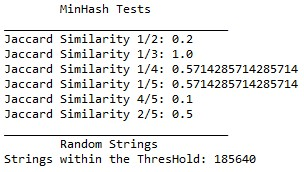
\includegraphics[width=150px]{teste_MinHash.jpg}
\caption{Teste - \textit{MinHash}}
\end{figure}
	
\begin{figure} [h]
\center
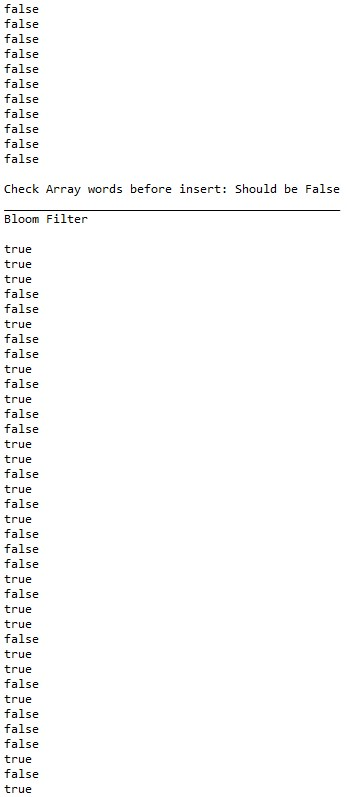
\includegraphics[width=150px]{teste1_BloomFilter.jpg}
\caption{Teste - \textit{Bloom Filter}}
\end{figure}

\begin{figure} [h]
\center
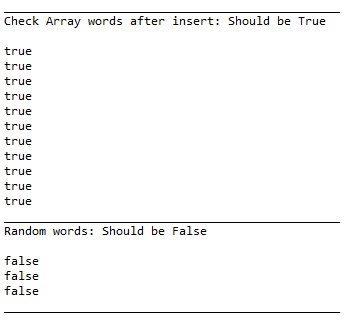
\includegraphics[width=150px]{teste2_BloomFilter.jpg}
\caption{Teste - \textit{Bloom Filter}}
\end{figure}

\begin{figure} [h]
\center
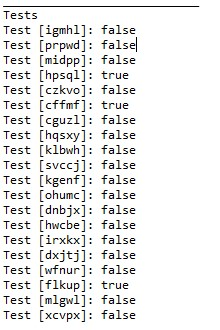
\includegraphics[width=150px]{test_bloom.jpg}
\caption{Teste - \textit{Bloom Filter}}
\end{figure}


%%%%%%%%%%%%%%%%%%%%%%%%%%%%%%%%%

\end{document}